\documentclass[a4paper,12pt]{ctexart} % 选择ctexart类
\usepackage{ctex} % 使用ctex包
\usepackage{amsmath} % 加载amsmath包
\usepackage{graphicx} % 支持插入图片
\usepackage{geometry} % 调整页面参数
\usepackage{booktabs}
\usepackage{float}
\geometry{a4paper,top=3cm,bottom=3cm,left=3cm,right=3cm}

\title{计算机组成原理第一次作业}
\author{}
\date{\today}
\begin{document}
	\maketitle
	\tableofcontents
	\section{企业雇佣画师创作图片}
	\subsection{请估算某企业雇佣一名画师进行一张图片创作成本}

在现代约稿市场中,绘画价格的差异很大,这种差异通常受到艺术家知名度、技能水平、作品的复杂度以及市场供需等多种因素的影响。工时是影响绘画成本的一个重要因素,因为创作一件作品所需的时间越长,其成本也越高,这包括了从构思、草稿到最终完成的整个过程。因此,在计算一幅绘画的成本时,我们会将工时纳入考虑,具体的计算方式如下:

设定绘画的成本公式为:
\[
\text{Cost} = \text{Drawing Time (hours)} \times \text{Hourly Wage}
\]

其中,时薪可以根据月薪计算得出:
\[
\text{Hourly Wage} = \frac{\text{Monthly Salary}}{22 \text{ days} \times 8 \text{ hours}}
\]

根据BOSS直聘APP对不同企业画师月薪的调查,我们整理了以下数据:

	\begin{tabular*}{25em}%
		{@{\extracolsep{\fill}}|c|c|c|}
		\hline
		公司 & 职位 & 月薪(人民币)  \\ \hline
		璃音网络 & 手绘卡画师 & 6000至7000  \\ 
		\hline
		普游天下&角色原画画师&13000至26000\\
		\hline
		火焰纹章 &游戏原画画师 &5000至10000\\
		\hline
		魔币科技&欧美Q版原画师&20000至30000\\
		\hline
		亿橙时代科技&资深游戏原画师&16000至18000\\
		\hline
		永航科技&2D角色原画师&13000至19000\\
		\hline
		光巢影视&二维卡通原画师&15000至30000\\
		\hline
	\end{tabular*}

根据上述数据,原画师的平均月薪约为:15571.42元
从而,平均时薪约为:88.47元
因此,一幅画的平均成本可以表示为:
\[
\text{Cost} = \text{Drawing Time (hours)} \times \text{88.47元}
\]
	\section{人工智能创作图片} 
	\subsection{请估算使用人工智能算法生成一张图片的成本}
	AI绘画,亦称AI艺术生成,是指运用人工智能技术创作视觉艺术作品的过程。它涉及多种AI技术,包括机器学习、深度学习、生成对抗网络(GANs)和变分自编码器(VAEs)。其中,机器学习与深度学习构成了AI绘画的基础,AI模型通过学习大量图像数据集来理解和模仿特定艺术风格或创造新的视觉内容。Stable Diffusion作为一种开源图像生成模型受到广泛关注,因其能够根据文本提示生成高分辨率、高质量的图像而备受推崇。

	AI绘画通常要求大量的计算资源,尤其是在训练阶段。随着生成器复杂度和图像分辨率的增加,所需的计算资源和时间也随之增长。这些资源包括专为并行处理设计的GPU,它们能够显著加速深度学习任务;以及用于高分辨率图像生成和模型训练的大量内存和数据存储空间。由于AI模型训练和运行会消耗大量能源,特别是在使用高性能计算资源时,能源成本也成为了不可忽视的重要因素。

	在讨论AI绘画成本时,我们以开源模型,Stable Diffusion,作为参考。原因在于,市场上大多数AI绘画公司往往不公开其财务报表和所采用的具体算法。这些公司可能使用专有技术,其成本结构和效率可能与公开可用的模型有所不同。然而,Stable Diffusion作为一种开源图像生成模型,不仅透明度高,而且在技术社区中得到了广泛的测试和应用,证明了其生成图像的质量和效率可以与许多闭源算法相媲美。

	为了计算使用Stable Diffusion生成一张图片的最低成本,我们需要考虑显卡的购买成本、功率消耗(电力成本)和算力。从Tom's Hardware提供的数据中,我们可以估算不同显卡生成一张512*512像素,50steps的图片的成本,进而确定AI绘画的最低成本。具体步骤包括:

	显卡摊销成本计算:
	假设显卡的预期使用寿命为3年,我们从AMD和NVIDIA的官网获取了不同显卡的官方指导价格,并以每年365天计算,总计1,095天。
\[
\text{Daily Amortized Cost} = \frac{\text{Price}}{\text{Lifespan (years)} \times 365}
\]

	电力成本计算:
	根据显卡的功率(W)和当地电价(每千瓦时的成本)计算。
\[
\text{Daily Power Cost} = \left(\frac{\text{Power}}{1000} \times \text{Electricity Cost (per kWh)}\right) \times \text{Hours per Day}
\]

算力计算:
使用Tom's Hardware提供的每分钟生成图像的数据估算每天可以生成的图片数量。
\begin{figure}[H]
\centering
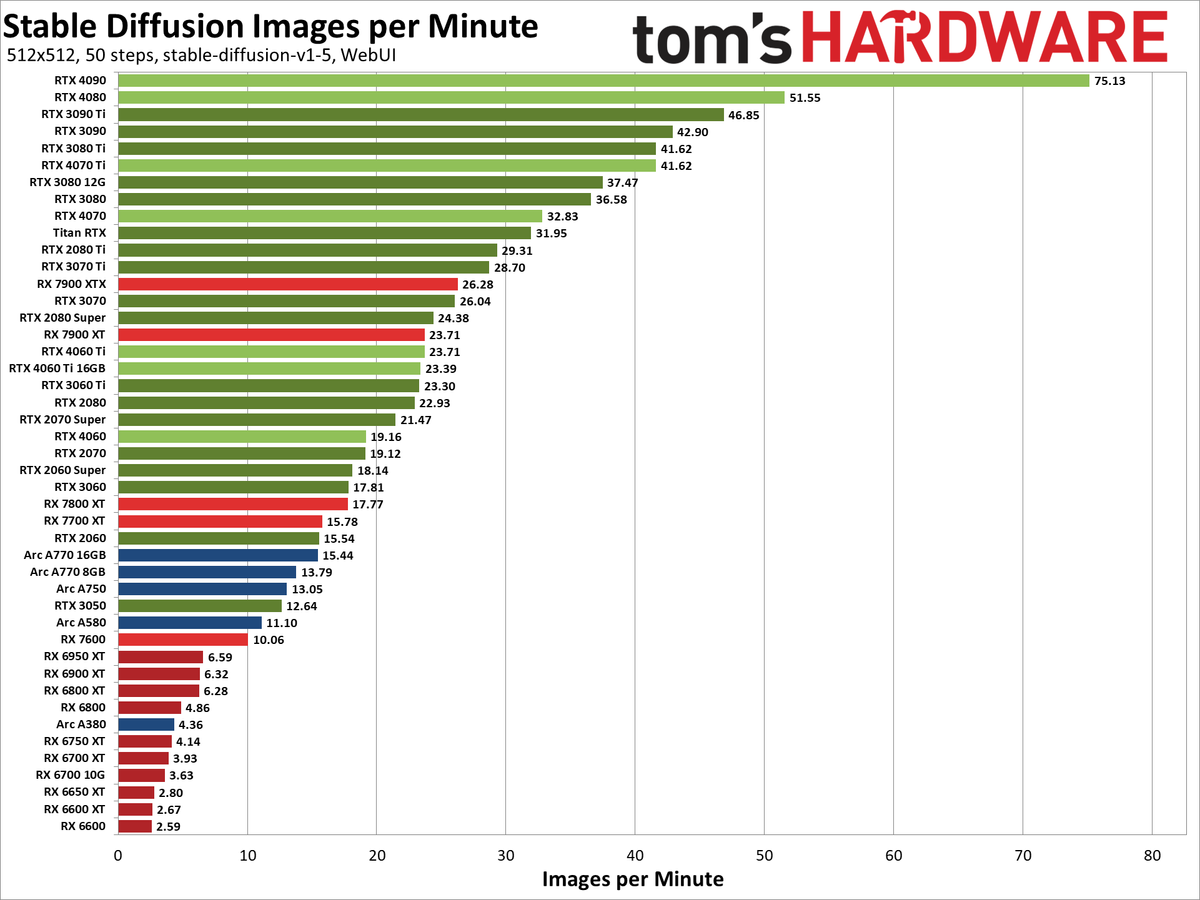
\includegraphics[width=0.8\textwidth]{images_per_minute.png}
\caption{Stable Diffusion Images per Minute}
\label{fig:example}
\end{figure}

	成本计算:
	将显卡的总生成量除以摊销成本和电力成本,得出每张图片的成本。
\[
\text{Cost Per Image} = \frac{\text{Daily Amortized Cost} + \text{Daily Power Cost}}{\text{Performance} \times \text{Hours per Day} \times 60}
\]	
在python中计算出数据后并将其可视化如下图所示
\begin{figure}[H]
\centering
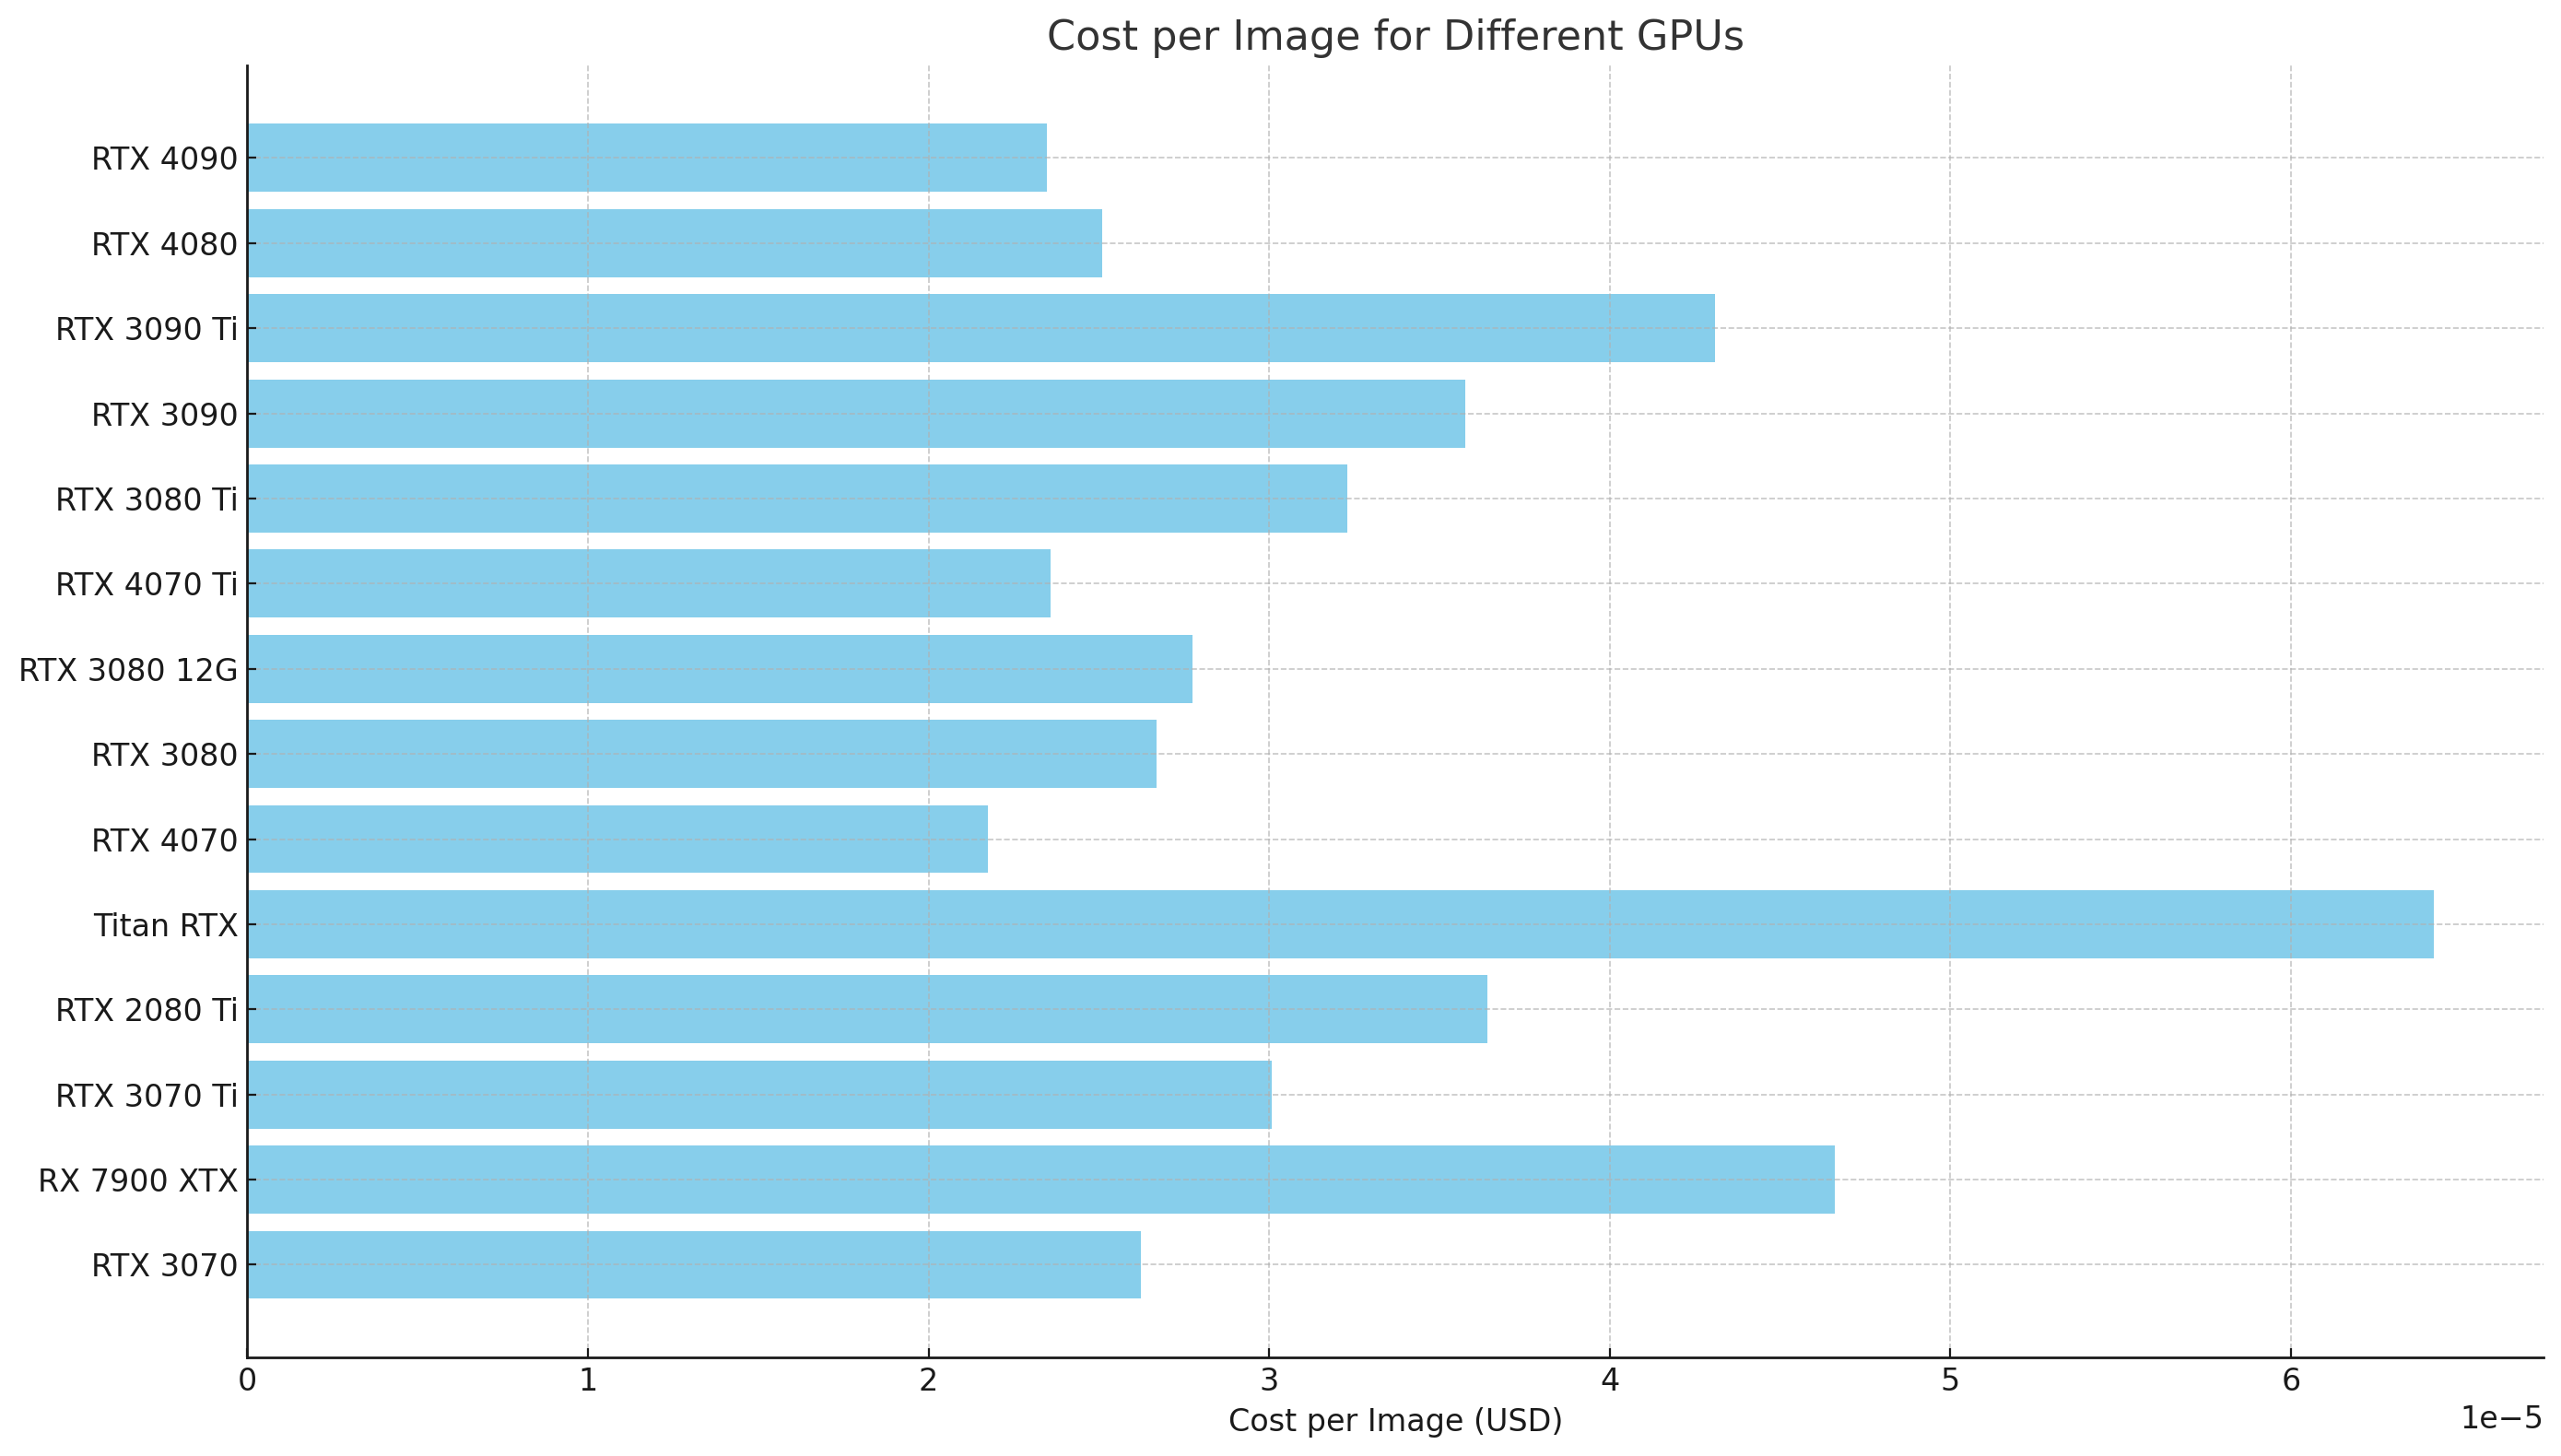
\includegraphics[width=0.8\textwidth]{cost_per_image.png}
\caption{Cost Per Image}
\label{fig:example}
\end{figure}

通过对比不同显卡的运行性能,我们发现虽然某些高端显卡在性能上领先,但价格适中的显卡在每张图片的成本效益上更有优势。例如,RTX 4070以合理的性能提供了最低的成本效益,每张图片的成本仅为0.0000217439美元。
	\section{结论与预测} 
	\subsection{从时间成本角度}从时间成本上AI占有巨大优势。人工智能绘画应用程序通过强大的算法和庞大的数据集,能够自动生成各种风格和风格的原画草图,从简笔画到写实风格,再到潮流的卡通风格,应有尽有,而每种风格的实现仅仅需要几分钟到几秒不等。而原画师不仅需要高超的绘画技术,也需要消耗大量的绘画精力,往往完成一幅画作需要几个小时甚至几天,和AI是远远不能相比的。AI绘画的出现让原画师面临着新的挑战。
	\subsection{从金钱成本角度}从金钱成本上AI同样也遥遥领先。目前大多数的绘画AI都是免费的价格,一部分具有限定的免费次数,只有少数需要直接付费,可见AI绘画及其便宜的金钱成本为原画师的生存岗位带来了极大的威胁。雇佣一名原画师的价格远远超过了AI的价格,这为公司如何选取作画手段起到了一定的引导作用。
	\subsection{AI亦有局限}当然AI并不是十全十美的。AI凭借一句话或几个关键字生成一幅完整的图画,显然无法满足设计者的所有需求,并且使用者不断的修改和调整也未必会实现想要达到的目标和效果。这时候原画师的作用就体现出来了。其可以借助AI绘画工具,迅速生成创意草图,节省大量的时间和精力。这种高效性让原画师能够再专注于创意的探索和设计的完善,为客户提供更具独特性的作品。而AI绘画在生成草图的同时,也能够通过学习人类创作的特点,帮助原画师再好地理解客户的需求,从而提供再贴合市场和受众的作品。
	\subsection{AI绘画是未来趋势}4.AI绘画对于数字绘画类岗位的影响是深远而复杂的。它既为原画、平面设计和插画带来了高效性和创意的拓展,也让从业者面临着新的挑战。对于数字绘画类岗位的从业者来说,不断学习和进步是必不可少的。只有不断拓展自己的技能和创作能力,与AI技术保持紧密结合,才能在未来的竞争中立于不败之地。AI绘画是数字绘画类岗位的未来趋势,让我们拥抱技术的力量,共同开创数字艺术的新纪元。
\end{document}